
Consider the standard variance component model described in lecture, with $K=6$, $J_i=5$ and $\{Y_{ij}\}$ the famous "dyestuff" date, with prior values $a_1=a_2=a_3=b_1=b_2=b_3=100$. Estimate the posterior mean of $W/V$, in each of the three ways:\\
(a) With a random-walk Metropolis algorithm.
Since we are dealing with likelihood functions, we need to compute things in log-scale. The ratio of distributions becomes $$\log\left(\frac{g(Y)}{g(X)}\right) = \log g(Y)-\log g(X)$$
The initial $\theta_i$ values are reasonably assumed to follow a normal distribution centered at sample mean of $Y_{ij}$ with $V,W$ equal to the sample variance of $Y_{ij}$. \\
The RWM algorithm is implemented as follows:
\begin{knitrout}
\definecolor{shadecolor}{rgb}{0.969, 0.969, 0.969}\color{fgcolor}\begin{kframe}
\begin{alltt}
\hlstd{a}\hlkwb{=}\hlnum{100}
\hlstd{K}\hlkwb{=}\hlnum{6}
\hlstd{J}\hlkwb{=}\hlnum{5}

\hlstd{B}\hlkwb{=}\hlnum{2e+6}
\hlstd{M}\hlkwb{=}\hlnum{5e+5}
\hlstd{sigma} \hlkwb{=} \hlnum{7}

\hlstd{Ydye} \hlkwb{=} \hlkwd{t}\hlstd{(} \hlkwd{matrix}\hlstd{(}
  \hlkwd{c}\hlstd{(}\hlnum{1545}\hlstd{,} \hlnum{1440}\hlstd{,} \hlnum{1440}\hlstd{,} \hlnum{1520}\hlstd{,} \hlnum{1580}\hlstd{,}
    \hlnum{1540}\hlstd{,} \hlnum{1555}\hlstd{,} \hlnum{1490}\hlstd{,} \hlnum{1560}\hlstd{,} \hlnum{1495}\hlstd{,}
    \hlnum{1595}\hlstd{,} \hlnum{1550}\hlstd{,} \hlnum{1605}\hlstd{,} \hlnum{1510}\hlstd{,} \hlnum{1560}\hlstd{,}
    \hlnum{1445}\hlstd{,} \hlnum{1440}\hlstd{,} \hlnum{1595}\hlstd{,} \hlnum{1465}\hlstd{,} \hlnum{1545}\hlstd{,}
    \hlnum{1595}\hlstd{,} \hlnum{1630}\hlstd{,} \hlnum{1515}\hlstd{,} \hlnum{1635}\hlstd{,} \hlnum{1625}\hlstd{,}
    \hlnum{1520}\hlstd{,} \hlnum{1455}\hlstd{,} \hlnum{1450}\hlstd{,} \hlnum{1480}\hlstd{,} \hlnum{1445}\hlstd{),} \hlkwc{nrow}\hlstd{=}\hlnum{5}\hlstd{) )}

\hlstd{logg} \hlkwb{=} \hlkwa{function}\hlstd{(}\hlkwc{m}\hlstd{,}\hlkwc{V}\hlstd{,}\hlkwc{W}\hlstd{,}\hlkwc{theta}\hlstd{,}\hlkwc{Ydye}\hlstd{) \{}
  \hlstd{g} \hlkwb{=} \hlopt{-}\hlstd{a}\hlopt{/}\hlstd{V} \hlopt{+} \hlkwd{log}\hlstd{(}\hlkwd{max}\hlstd{(}\hlkwd{c}\hlstd{(V,}\hlnum{1e-5}\hlstd{)))}\hlopt{*}\hlstd{(}\hlopt{-}\hlstd{a}\hlopt{-}\hlnum{1}\hlstd{)} \hlopt{+} \hlstd{(}\hlopt{-}\hlstd{a}\hlopt{/}\hlstd{W)}
  \hlstd{g} \hlkwb{=} \hlstd{g} \hlopt{+} \hlkwd{log}\hlstd{(}\hlkwd{max}\hlstd{(}\hlkwd{c}\hlstd{(W,}\hlnum{1e-5}\hlstd{)))}\hlopt{*}\hlstd{(}\hlopt{-}\hlstd{a}\hlopt{-}\hlnum{1}\hlstd{)} \hlopt{-} \hlstd{(m}\hlopt{-}\hlstd{a)}\hlopt{^}\hlnum{2}\hlopt{/}\hlstd{a}\hlopt{/}\hlnum{2}
  \hlstd{g} \hlkwb{=} \hlstd{g} \hlopt{+} \hlkwd{log}\hlstd{(}\hlkwd{max}\hlstd{(}\hlkwd{c}\hlstd{(V,}\hlnum{1e-5}\hlstd{)))}\hlopt{*}\hlstd{(}\hlopt{-}\hlstd{K}\hlopt{/}\hlnum{2}\hlstd{)} \hlopt{+} \hlkwd{log}\hlstd{(}\hlkwd{max}\hlstd{(}\hlkwd{c}\hlstd{(W,}\hlnum{1e-5}\hlstd{)))}\hlopt{*}\hlstd{(}\hlopt{-}\hlstd{K}\hlopt{*}\hlstd{J}\hlopt{/}\hlnum{2}\hlstd{)}
  \hlstd{g} \hlkwb{=} \hlstd{g} \hlopt{-} \hlkwd{sum}\hlstd{((theta}\hlopt{-}\hlstd{m)}\hlopt{^}\hlnum{2}\hlstd{)}\hlopt{/}\hlstd{V}\hlopt{/}\hlnum{2} \hlopt{-} \hlkwd{sum}\hlstd{((Ydye}\hlopt{-}\hlstd{theta)}\hlopt{^}\hlnum{2}\hlstd{)}\hlopt{/}\hlstd{W}\hlopt{/}\hlnum{2}
  \hlkwd{return} \hlstd{(g)}
\hlstd{\}}

\hlstd{m} \hlkwb{=} \hlkwd{rnorm}\hlstd{(}\hlnum{1}\hlstd{,a,a)}
\hlstd{V} \hlkwb{=} \hlkwd{var}\hlstd{(}\hlkwd{c}\hlstd{(Ydye))}
\hlstd{W} \hlkwb{=} \hlkwd{var}\hlstd{(}\hlkwd{c}\hlstd{(Ydye))}
\hlstd{theta} \hlkwb{=} \hlkwd{rnorm}\hlstd{(K,}\hlkwd{mean}\hlstd{(Ydye),}\hlkwd{sqrt}\hlstd{(V))}
\hlstd{acc} \hlkwb{=} \hlnum{0}
\hlstd{fnlist} \hlkwb{=} \hlkwd{numeric}\hlstd{(B}\hlopt{+}\hlstd{M)}

\hlkwa{for} \hlstd{(i} \hlkwa{in} \hlnum{1}\hlopt{:}\hlstd{(B}\hlopt{+}\hlstd{M)) \{}
  \hlstd{eps_m} \hlkwb{=} \hlkwd{rnorm}\hlstd{(}\hlnum{1}\hlstd{,}\hlnum{0}\hlstd{,sigma)}
  \hlstd{eps_V} \hlkwb{=} \hlkwd{rnorm}\hlstd{(}\hlnum{1}\hlstd{,}\hlnum{0}\hlstd{,sigma)}
  \hlstd{eps_W} \hlkwb{=} \hlkwd{rnorm}\hlstd{(}\hlnum{1}\hlstd{,}\hlnum{0}\hlstd{,sigma)}
  \hlstd{eps_theta} \hlkwb{=} \hlkwd{rnorm}\hlstd{(K,}\hlnum{0}\hlstd{,sigma)}

  \hlstd{dg} \hlkwb{=} \hlkwd{logg}\hlstd{(m}\hlopt{+}\hlstd{eps_m,V}\hlopt{+}\hlstd{eps_V,W}\hlopt{+}\hlstd{eps_W,theta}\hlopt{+}\hlstd{eps_theta,Ydye)} \hlopt{-}
    \hlkwd{logg}\hlstd{(m,V,W,theta,Ydye)}
  \hlkwa{if} \hlstd{(}\hlkwd{runif}\hlstd{(}\hlnum{1}\hlstd{)}\hlopt{<=}\hlkwd{exp}\hlstd{(dg)) \{}
    \hlkwa{if} \hlstd{(i}\hlopt{>}\hlstd{B)}
      \hlstd{acc} \hlkwb{=} \hlstd{acc} \hlopt{+} \hlnum{1}
    \hlstd{m} \hlkwb{=} \hlstd{m}\hlopt{+}\hlstd{eps_m}
    \hlstd{V} \hlkwb{=} \hlstd{V}\hlopt{+}\hlstd{eps_V}
    \hlstd{W} \hlkwb{=} \hlstd{W}\hlopt{+}\hlstd{eps_W}
    \hlstd{theta} \hlkwb{=} \hlstd{theta}\hlopt{+}\hlstd{eps_theta}
  \hlstd{\}}
  \hlstd{fnlist[i]} \hlkwb{=} \hlstd{W}\hlopt{/}\hlstd{V}
\hlstd{\}}
\hlstd{funcmean} \hlkwb{=} \hlkwd{mean}\hlstd{(fnlist[(B}\hlopt{+}\hlnum{1}\hlstd{)}\hlopt{:}\hlstd{(M}\hlopt{+}\hlstd{B)])}
\hlstd{funciidse} \hlkwb{=} \hlkwd{sd}\hlstd{(fnlist[(B}\hlopt{+}\hlnum{1}\hlstd{)}\hlopt{:}\hlstd{(M}\hlopt{+}\hlstd{B)])}\hlopt{/}\hlkwd{sqrt}\hlstd{(M)}
\hlstd{acf_k} \hlkwb{=} \hlkwd{acf}\hlstd{(fnlist[(B}\hlopt{+}\hlnum{1}\hlstd{)}\hlopt{:}\hlstd{(M}\hlopt{+}\hlstd{B)],}\hlkwc{lag.max} \hlstd{=} \hlnum{1000}\hlstd{,}\hlkwc{plot} \hlstd{=} \hlnum{FALSE}\hlstd{)}\hlopt{$}\hlstd{acf}
\hlstd{varfact} \hlkwb{=} \hlnum{2}\hlopt{*}\hlkwd{sum}\hlstd{(acf_k)}\hlopt{-}\hlnum{1}
\hlstd{funcse} \hlkwb{=} \hlstd{funciidse}\hlopt{*}\hlkwd{sqrt}\hlstd{(varfact)}
\hlstd{accrate} \hlkwb{=} \hlstd{acc}\hlopt{/}\hlstd{M}

\hlkwd{cat}\hlstd{(}\hlstr{'B = '}\hlstd{,B,}\hlstr{', M = '}\hlstd{,M,}\hlstr{'\textbackslash{}n'}\hlstd{)}
\hlkwd{cat}\hlstd{(}\hlstr{'Number of samples accepted = '}\hlstd{,acc,}\hlstr{', acceptance rate = '}\hlstd{,accrate,}\hlstr{'\textbackslash{}n'}\hlstd{)}
\hlkwd{cat}\hlstd{(}\hlstr{'Estimate = '}\hlstd{,funcmean,}\hlstr{'\textbackslash{}n'}\hlstd{)}
\hlkwd{cat}\hlstd{(}\hlstr{'i.i.d. standard error = '}\hlstd{,funciidse,}\hlstr{'\textbackslash{}n'}\hlstd{)}
\hlkwd{cat}\hlstd{(}\hlstr{'varfact = '}\hlstd{,varfact,}\hlstr{'\textbackslash{}n'}\hlstd{)}
\hlkwd{cat}\hlstd{(}\hlstr{'Standard error = '}\hlstd{,funcse,}\hlstr{'\textbackslash{}n'}\hlstd{)}
\end{alltt}
\end{kframe}
\end{knitrout}
Output of several runs:
\begin{knitrout}
\definecolor{shadecolor}{rgb}{0.969, 0.969, 0.969}\color{fgcolor}\begin{kframe}
\begin{verbatim}
## B =  2e+06 , M =  5e+05 
## Number of samples accepted =  127952 , acceptance rate =  0.255904 
## Estimate =  0.006394276 
## i.i.d. standard error =  8.691605e-07 
## varfact =  222.6512 
## Standard error =  1.296918e-05
## B =  2e+06 , M =  5e+05 
## Number of samples accepted =  127690 , acceptance rate =  0.25538 
## Estimate =  0.005920185 
## i.i.d. standard error =  8.150501e-07 
## varfact =  259.4071 
## Standard error =  1.312729e-05
## B =  2e+06 , M =  5e+05 
## Number of samples accepted =  127896 , acceptance rate =  0.255792 
## Estimate =  0.006361079 
## i.i.d. standard error =  8.695236e-07 
## varfact =  242.357 
## Standard error =  1.353659e-05
## B =  2e+06 , M =  5e+05 
## Number of samples accepted =  127489 , acceptance rate =  0.254978 
## Estimate =  0.006515764 
## i.i.d. standard error =  9.252959e-07 
## varfact =  382.6875 
## Standard error =  1.810101e-05
## B =  2e+06 , M =  5e+05 
## Number of samples accepted =  128078 , acceptance rate =  0.256156 
## Estimate =  0.005825482 
## i.i.d. standard error =  8.563688e-07 
## varfact =  477.4472 
## Standard error =  1.871214e-05
\end{verbatim}
\end{kframe}
\end{knitrout}
The tabulated result is as follows:\\
\begin{center}
\begin{knitrout}
\definecolor{shadecolor}{rgb}{0.969, 0.969, 0.969}\color{fgcolor}
\begin{tabular}{r|r|r|r|r}
\hline
estimation & acc\_rate & seiid & varfact\_r & standard\_error\\
\hline
0.0063943 & 0.255904 & 9e-07 & 222.6512 & 1.30e-05\\
\hline
0.0059202 & 0.255380 & 8e-07 & 259.4071 & 1.31e-05\\
\hline
0.0063611 & 0.255792 & 9e-07 & 242.3570 & 1.35e-05\\
\hline
0.0065158 & 0.254978 & 9e-07 & 382.6875 & 1.81e-05\\
\hline
0.0058255 & 0.256156 & 9e-07 & 477.4472 & 1.87e-05\\
\hline
\end{tabular}


\end{knitrout}
\end{center}

\begin{figure}[H]
  \centering
\begin{knitrout}
\definecolor{shadecolor}{rgb}{0.969, 0.969, 0.969}\color{fgcolor}\begin{kframe}
\begin{alltt}
\hlkwd{plot}\hlstd{(fnlist[(B}\hlopt{+}\hlnum{1}\hlstd{)}\hlopt{:}\hlstd{(B}\hlopt{+}\hlstd{M)],}\hlkwc{type}\hlstd{=}\hlstr{'l'}\hlstd{)}
\end{alltt}
\end{kframe}
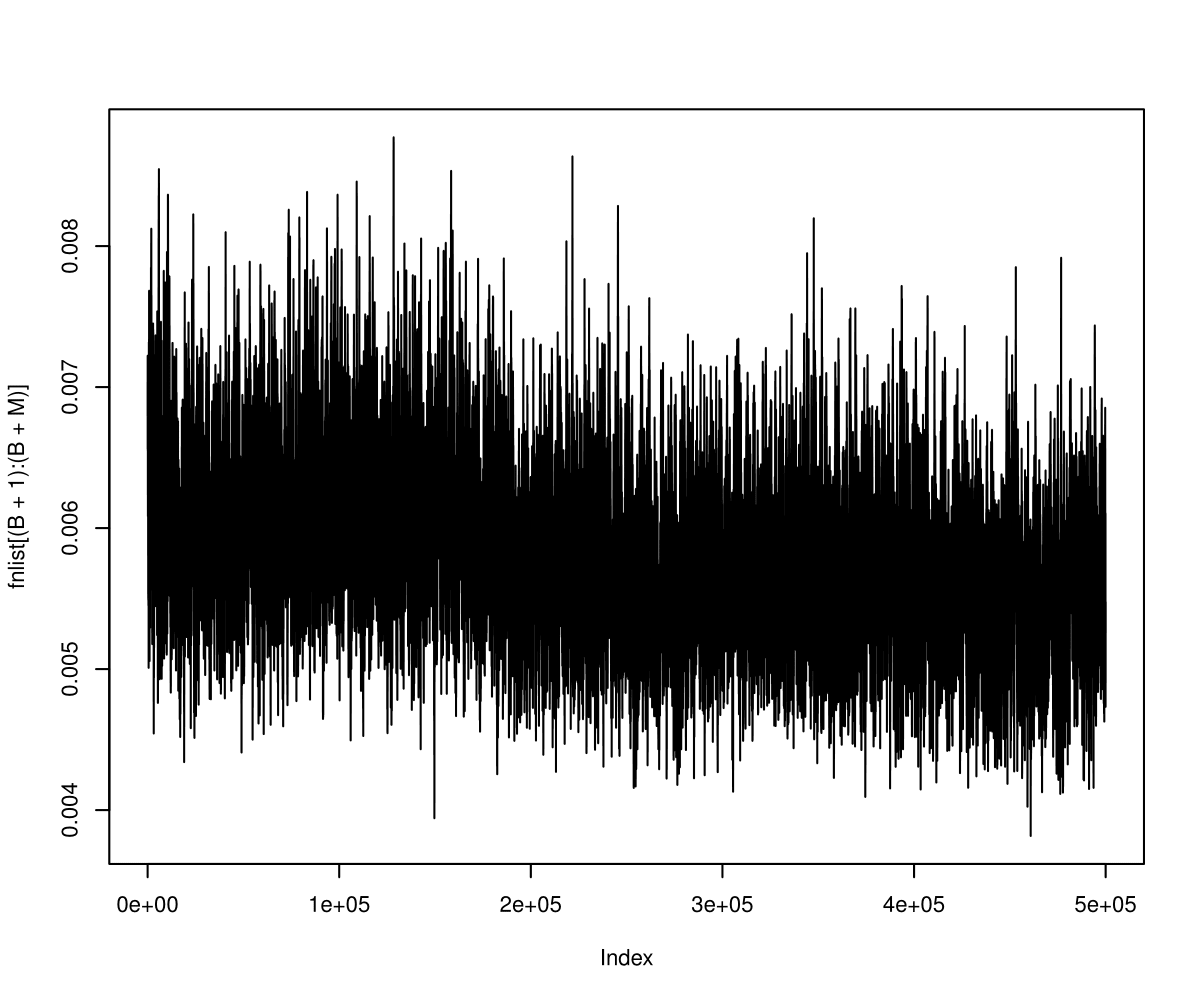
\includegraphics[width=\maxwidth]{figure/p9aplot-1} 

\end{knitrout}
		\caption{function values of Random-Walk Metropolis algorithm after burning-in}
\end{figure}
(b) With a Metropolis-within-Gibbs algorithm.
Using a Metropolis-within-Gibbs algorithem, we can safely increase $\sigma$. Source code:

\begin{knitrout}
\definecolor{shadecolor}{rgb}{0.969, 0.969, 0.969}\color{fgcolor}\begin{kframe}
\begin{alltt}
\hlstd{a}\hlkwb{=}\hlnum{100}
\hlstd{K}\hlkwb{=}\hlnum{6}
\hlstd{J}\hlkwb{=}\hlnum{5}

\hlstd{B}\hlkwb{=}\hlnum{1e+6}
\hlstd{M}\hlkwb{=}\hlnum{5e+5}
\hlstd{sigma} \hlkwb{=} \hlnum{40}

\hlstd{Ydye} \hlkwb{=} \hlkwd{t}\hlstd{(} \hlkwd{matrix}\hlstd{(}
  \hlkwd{c}\hlstd{(}\hlnum{1545}\hlstd{,} \hlnum{1440}\hlstd{,} \hlnum{1440}\hlstd{,} \hlnum{1520}\hlstd{,} \hlnum{1580}\hlstd{,}
    \hlnum{1540}\hlstd{,} \hlnum{1555}\hlstd{,} \hlnum{1490}\hlstd{,} \hlnum{1560}\hlstd{,} \hlnum{1495}\hlstd{,}
    \hlnum{1595}\hlstd{,} \hlnum{1550}\hlstd{,} \hlnum{1605}\hlstd{,} \hlnum{1510}\hlstd{,} \hlnum{1560}\hlstd{,}
    \hlnum{1445}\hlstd{,} \hlnum{1440}\hlstd{,} \hlnum{1595}\hlstd{,} \hlnum{1465}\hlstd{,} \hlnum{1545}\hlstd{,}
    \hlnum{1595}\hlstd{,} \hlnum{1630}\hlstd{,} \hlnum{1515}\hlstd{,} \hlnum{1635}\hlstd{,} \hlnum{1625}\hlstd{,}
    \hlnum{1520}\hlstd{,} \hlnum{1455}\hlstd{,} \hlnum{1450}\hlstd{,} \hlnum{1480}\hlstd{,} \hlnum{1445}\hlstd{),} \hlkwc{nrow}\hlstd{=}\hlnum{5}\hlstd{) )}

\hlstd{logg} \hlkwb{=} \hlkwa{function}\hlstd{(}\hlkwc{m}\hlstd{,}\hlkwc{V}\hlstd{,}\hlkwc{W}\hlstd{,}\hlkwc{theta}\hlstd{,}\hlkwc{Ydye}\hlstd{) \{}
  \hlstd{g} \hlkwb{=} \hlopt{-}\hlstd{a}\hlopt{/}\hlstd{V} \hlopt{+} \hlkwd{log}\hlstd{(}\hlkwd{max}\hlstd{(}\hlkwd{c}\hlstd{(V,}\hlnum{1e-5}\hlstd{)))}\hlopt{*}\hlstd{(}\hlopt{-}\hlstd{a}\hlopt{-}\hlnum{1}\hlstd{)} \hlopt{+} \hlstd{(}\hlopt{-}\hlstd{a}\hlopt{/}\hlstd{W)}
  \hlstd{g} \hlkwb{=} \hlstd{g} \hlopt{+} \hlkwd{log}\hlstd{(}\hlkwd{max}\hlstd{(}\hlkwd{c}\hlstd{(W,}\hlnum{1e-5}\hlstd{)))}\hlopt{*}\hlstd{(}\hlopt{-}\hlstd{a}\hlopt{-}\hlnum{1}\hlstd{)} \hlopt{-} \hlstd{(m}\hlopt{-}\hlstd{a)}\hlopt{^}\hlnum{2}\hlopt{/}\hlstd{a}\hlopt{/}\hlnum{2}
  \hlstd{g} \hlkwb{=} \hlstd{g} \hlopt{+} \hlkwd{log}\hlstd{(}\hlkwd{max}\hlstd{(}\hlkwd{c}\hlstd{(V,}\hlnum{1e-5}\hlstd{)))}\hlopt{*}\hlstd{(}\hlopt{-}\hlstd{K}\hlopt{/}\hlnum{2}\hlstd{)} \hlopt{+} \hlkwd{log}\hlstd{(}\hlkwd{max}\hlstd{(}\hlkwd{c}\hlstd{(W,}\hlnum{1e-5}\hlstd{)))}\hlopt{*}\hlstd{(}\hlopt{-}\hlstd{K}\hlopt{*}\hlstd{J}\hlopt{/}\hlnum{2}\hlstd{)}
  \hlstd{g} \hlkwb{=} \hlstd{g} \hlopt{-} \hlkwd{sum}\hlstd{((theta}\hlopt{-}\hlstd{m)}\hlopt{^}\hlnum{2}\hlstd{)}\hlopt{/}\hlstd{V}\hlopt{/}\hlnum{2} \hlopt{-} \hlkwd{sum}\hlstd{((Ydye}\hlopt{-}\hlstd{theta)}\hlopt{^}\hlnum{2}\hlstd{)}\hlopt{/}\hlstd{W}\hlopt{/}\hlnum{2}
  \hlkwd{return} \hlstd{(g)}
\hlstd{\}}

\hlstd{m} \hlkwb{=} \hlkwd{rnorm}\hlstd{(}\hlnum{1}\hlstd{,a,sigma)}
\hlstd{V} \hlkwb{=} \hlkwd{var}\hlstd{(}\hlkwd{c}\hlstd{(Ydye))}
\hlstd{W} \hlkwb{=} \hlkwd{var}\hlstd{(}\hlkwd{c}\hlstd{(Ydye))}
\hlstd{theta} \hlkwb{=} \hlkwd{rnorm}\hlstd{(K,}\hlkwd{mean}\hlstd{(Ydye),}\hlkwd{sqrt}\hlstd{(V))}
\hlstd{acc} \hlkwb{=} \hlnum{0}
\hlstd{fnlist} \hlkwb{=} \hlkwd{numeric}\hlstd{(B}\hlopt{+}\hlstd{M)}

\hlkwa{for} \hlstd{(i} \hlkwa{in} \hlnum{1}\hlopt{:}\hlstd{(B}\hlopt{+}\hlstd{M)) \{}
  \hlstd{eps_m}\hlkwb{=}\hlnum{0}
  \hlstd{eps_V}\hlkwb{=}\hlnum{0}
  \hlstd{eps_W}\hlkwb{=}\hlnum{0}
  \hlstd{eps_theta} \hlkwb{=} \hlkwd{rep}\hlstd{(}\hlnum{0}\hlstd{,K)}
  \hlstd{ci} \hlkwb{=} \hlstd{i} \hlopt \hlstd{(}\hlnum{3}\hlopt{+}\hlstd{K)}
  \hlkwa{if} \hlstd{(ci}\hlopt{==}\hlnum{0}\hlstd{)}
    \hlstd{eps_m} \hlkwb{=} \hlkwd{rnorm}\hlstd{(}\hlnum{1}\hlstd{,}\hlnum{0}\hlstd{,sigma)}
  \hlkwa{else if} \hlstd{(ci}\hlopt{==}\hlnum{1}\hlstd{)}
    \hlstd{eps_V} \hlkwb{=} \hlkwd{rnorm}\hlstd{(}\hlnum{1}\hlstd{,}\hlnum{0}\hlstd{,sigma)}
  \hlkwa{else if} \hlstd{(ci}\hlopt{==}\hlnum{2}\hlstd{)}
    \hlstd{eps_W} \hlkwb{=} \hlkwd{rnorm}\hlstd{(}\hlnum{1}\hlstd{,}\hlnum{0}\hlstd{,sigma)}
  \hlkwa{else}
    \hlstd{eps_theta[ci}\hlopt{-}\hlnum{2}\hlstd{]} \hlkwb{=} \hlkwd{rnorm}\hlstd{(}\hlnum{1}\hlstd{,}\hlnum{0}\hlstd{,sigma)}

  \hlstd{dg} \hlkwb{=} \hlkwd{logg}\hlstd{(m}\hlopt{+}\hlstd{eps_m,V}\hlopt{+}\hlstd{eps_V,W}\hlopt{+}\hlstd{eps_W,theta}\hlopt{+}\hlstd{eps_theta,Ydye)} \hlopt{-}
    \hlkwd{logg}\hlstd{(m,V,W,theta,Ydye)}
  \hlkwa{if} \hlstd{(}\hlkwd{runif}\hlstd{(}\hlnum{1}\hlstd{)}\hlopt{<=}\hlkwd{exp}\hlstd{(dg)) \{}
    \hlkwa{if} \hlstd{(i}\hlopt{>}\hlstd{B)}
    \hlstd{acc} \hlkwb{=} \hlstd{acc} \hlopt{+} \hlnum{1}
    \hlstd{m} \hlkwb{=} \hlstd{m}\hlopt{+}\hlstd{eps_m}
    \hlstd{V} \hlkwb{=} \hlstd{V}\hlopt{+}\hlstd{eps_V}
    \hlstd{W} \hlkwb{=} \hlstd{W}\hlopt{+}\hlstd{eps_W}
    \hlstd{theta} \hlkwb{=} \hlstd{theta}\hlopt{+}\hlstd{eps_theta}
  \hlstd{\}}
  \hlstd{fnlist[i]} \hlkwb{=} \hlstd{W}\hlopt{/}\hlstd{V}
\hlstd{\}}
\hlstd{funcmean} \hlkwb{=} \hlkwd{mean}\hlstd{(fnlist[(B}\hlopt{+}\hlnum{1}\hlstd{)}\hlopt{:}\hlstd{(M}\hlopt{+}\hlstd{B)])}
\hlstd{funciidse} \hlkwb{=} \hlkwd{sd}\hlstd{(fnlist[(B}\hlopt{+}\hlnum{1}\hlstd{)}\hlopt{:}\hlstd{(M}\hlopt{+}\hlstd{B)])}\hlopt{/}\hlkwd{sqrt}\hlstd{(M)}
\hlstd{acf_k} \hlkwb{=} \hlkwd{acf}\hlstd{(fnlist[(B}\hlopt{+}\hlnum{1}\hlstd{)}\hlopt{:}\hlstd{(M}\hlopt{+}\hlstd{B)],}\hlkwc{lag.max} \hlstd{=} \hlnum{1000}\hlstd{,}\hlkwc{plot} \hlstd{=} \hlnum{FALSE}\hlstd{)}\hlopt{$}\hlstd{acf}
\hlstd{varfact} \hlkwb{=} \hlnum{2}\hlopt{*}\hlkwd{sum}\hlstd{(acf_k)}\hlopt{-}\hlnum{1}
\hlstd{funcse} \hlkwb{=} \hlstd{funciidse}\hlopt{*}\hlkwd{sqrt}\hlstd{(varfact)}
\hlstd{accrate} \hlkwb{=} \hlstd{acc}\hlopt{/}\hlstd{M}

\hlkwd{cat}\hlstd{(}\hlstr{'B = '}\hlstd{,B,}\hlstr{', M = '}\hlstd{,M,}\hlstr{'\textbackslash{}n'}\hlstd{)}
\hlkwd{cat}\hlstd{(}\hlstr{'Number of samples accepted = '}\hlstd{,acc,}\hlstr{', acceptance rate = '}\hlstd{,accrate,}\hlstr{'\textbackslash{}n'}\hlstd{)}
\hlkwd{cat}\hlstd{(}\hlstr{'Estimate = '}\hlstd{,funcmean,}\hlstr{'\textbackslash{}n'}\hlstd{)}
\hlkwd{cat}\hlstd{(}\hlstr{'i.i.d. standard error = '}\hlstd{,funciidse,}\hlstr{'\textbackslash{}n'}\hlstd{)}
\hlkwd{cat}\hlstd{(}\hlstr{'varfact = '}\hlstd{,varfact,}\hlstr{'\textbackslash{}n'}\hlstd{)}
\hlkwd{cat}\hlstd{(}\hlstr{'Standard error = '}\hlstd{,funcse,}\hlstr{'\textbackslash{}n'}\hlstd{)}
\end{alltt}
\end{kframe}
\end{knitrout}
Output of several runs:
\begin{knitrout}
\definecolor{shadecolor}{rgb}{0.969, 0.969, 0.969}\color{fgcolor}\begin{kframe}
\begin{verbatim}
## B =  1e+06 , M =  5e+05 
## Number of samples accepted =  177717 , acceptance rate =  0.355434 
## Estimate =  0.005133218 
## i.i.d. standard error =  7.382176e-07 
## varfact =  298.7258 
## Standard error =  1.275912e-05
## B =  1e+06 , M =  5e+05 
## Number of samples accepted =  177155 , acceptance rate =  0.35431 
## Estimate =  0.004777328 
## i.i.d. standard error =  7.062485e-07 
## varfact =  357.6378 
## Standard error =  1.335609e-05
## B =  1e+06 , M =  5e+05 
## Number of samples accepted =  177056 , acceptance rate =  0.354112 
## Estimate =  0.004697013 
## i.i.d. standard error =  6.735418e-07 
## varfact =  305.6105 
## Standard error =  1.177467e-05
## B =  1e+06 , M =  5e+05 
## Number of samples accepted =  177643 , acceptance rate =  0.355286 
## Estimate =  0.004896768 
## i.i.d. standard error =  8.344297e-07 
## varfact =  779.2573 
## Standard error =  2.329326e-05
## B =  1e+06 , M =  5e+05 
## Number of samples accepted =  177505 , acceptance rate =  0.35501 
## Estimate =  0.004181851 
## i.i.d. standard error =  6.293576e-07 
## varfact =  411.9449 
## Standard error =  1.277371e-05
\end{verbatim}
\end{kframe}
\end{knitrout}
The tabulated result is as follows:\\
\begin{center}
\begin{knitrout}
\definecolor{shadecolor}{rgb}{0.969, 0.969, 0.969}\color{fgcolor}
\begin{tabular}{r|r|r|r|r}
\hline
estimation & acc\_rate & seiid & varfact\_r & standard\_error\\
\hline
0.0051332 & 0.355434 & 7e-07 & 298.7258 & 1.28e-05\\
\hline
0.0047773 & 0.354310 & 7e-07 & 357.6378 & 1.34e-05\\
\hline
0.0046970 & 0.354112 & 7e-07 & 305.6105 & 1.18e-05\\
\hline
0.0048968 & 0.355286 & 8e-07 & 779.2573 & 2.33e-05\\
\hline
0.0041819 & 0.355010 & 6e-07 & 411.9449 & 1.28e-05\\
\hline
\end{tabular}


\end{knitrout}
\end{center}
\begin{figure}[H]
  \centering
\begin{knitrout}
\definecolor{shadecolor}{rgb}{0.969, 0.969, 0.969}\color{fgcolor}\begin{kframe}
\begin{alltt}
\hlkwd{plot}\hlstd{(fnlist[(B}\hlopt{+}\hlnum{1}\hlstd{)}\hlopt{:}\hlstd{(B}\hlopt{+}\hlstd{M)],}\hlkwc{type}\hlstd{=}\hlstr{'l'}\hlstd{)}
\end{alltt}
\end{kframe}
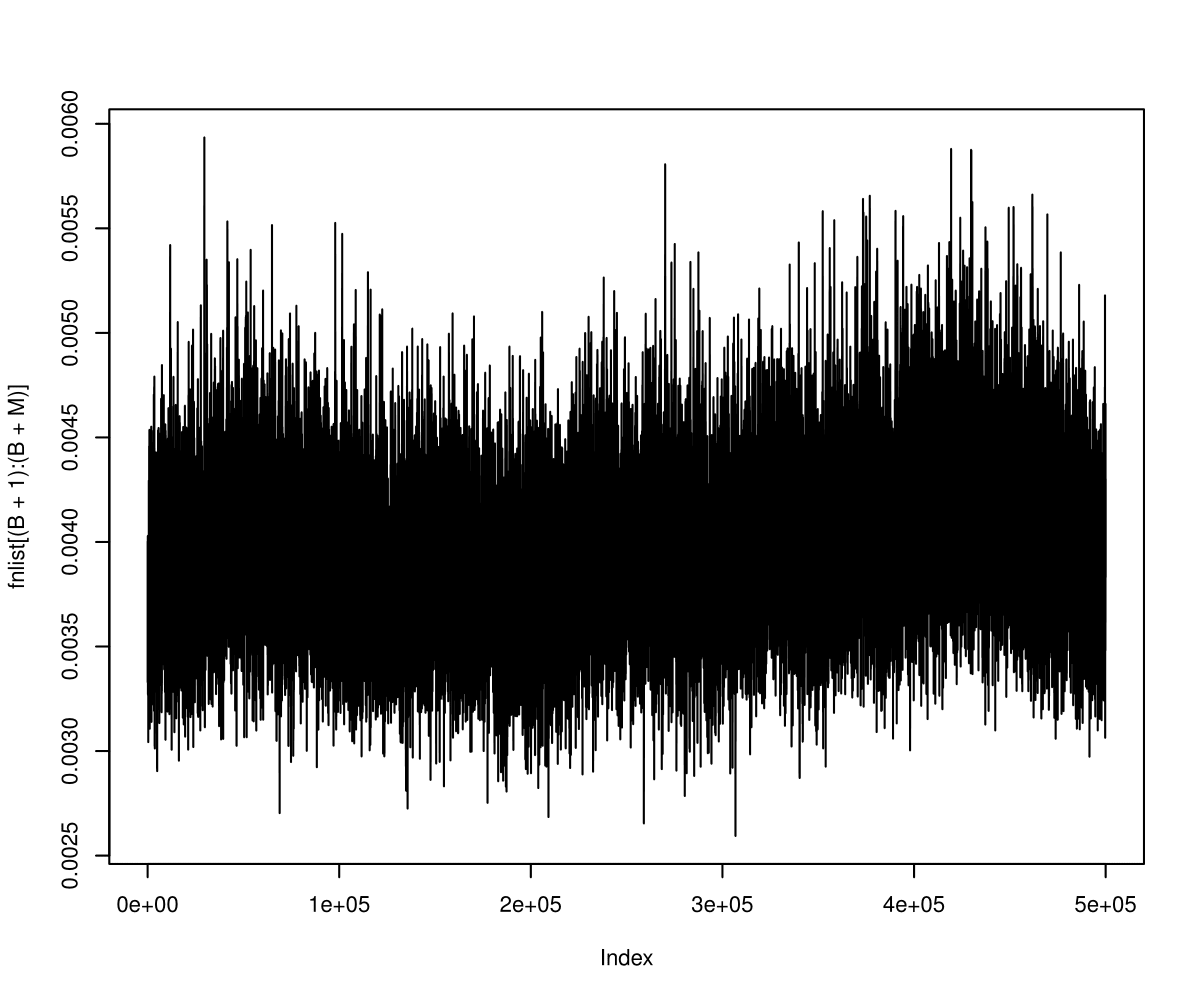
\includegraphics[width=\maxwidth]{figure/p9bplot-1} 

\end{knitrout}
		\caption{function values of Metropolis-within-Gibbs algorithm after burning-in}
\end{figure}
(c) With a Gibbs sampler.\\
For Gibbs sampler, we need to calculate the conditional distributions in closed form. \\
Firstly, the joint distribution is given by 
\begin{align*}
f(V,W,\mu,\theta,Y) = &Ce^{-b_1/V}V^{-a_1-1}e^{-b_2/W}W^{-a_2-1}e^{-(\mu-a3)^2/2b_3}V^{-K/2}W^{-\frac{1}{2}KJ}\times\\
                      &\exp\left[-\sum\limits_{i=1}^K(\theta_i-\mu)^2/2V - \sum\limits_{i=1}^K\sum\limits_{j=1}^J(Y_{ij}-\theta_i)^2/2W\right]\\
                       = &Ce^{-a/V}V^{-a-1}e^{-a/W}W^{-a-1}e^{-(\mu-a)^2/2a}V^{-K/2}W^{-\frac{1}{2}KJ}\times\\
                      &\exp\left[-\sum\limits_{i=1}^K(\theta_i-\mu)^2/2V - \sum\limits_{i=1}^K\sum\limits_{j=1}^J(Y_{ij}-\theta_i)^2/2W\right]
\end{align*}
where C is a normalizing constant, and $a=a_1=a_2=a_3=b_1=b_2=b_3$. \\
Now, we can write the following conditional distributions:
\begin{align*}
f(\mu|V,W,\theta) &= C\exp\left[-\frac{(\mu-a)^2}{2a}-\sum\limits_{i=1}^K\frac{(\theta_i-\mu)^2}{2V}\right]\\
    &= C\exp\left[-\mu^2\left(\frac{1}{2a}+\frac{K}{2V}\right)+\mu\left(1+\sum\limits_{i=1}^K\frac{\theta_i}{V}\right)\right]\\
\end{align*}
If we let $\mu|*$ to follow a $N(m,v)$ distribution for some $m$ and $v$, and match the coefficients to get
$$v=\left(\frac{1}{2a}+\frac{K}{2V}\right)^{-1}\bigg/2 = \left(\frac{1}{a}+\frac{K}{V}\right)^{-1}$$
$$m=\left(1+\sum\limits_{i=1}^K\frac{\theta_i}{V}\right)\left(\frac{1}{a}+\frac{K}{V}\right)^{-1}$$
Therefore, we have 
$$(\mu|V,W,\theta)\sim N\left(\left(1+\sum\limits_{i=1}^K\frac{\theta_i}{V}\right)\left(\frac{1}{a}+\frac{K}{V}\right)^{-1},\left(\frac{1}{a}+\frac{K}{V}\right)^{-1}\right)$$
\begin{align*}
f(V|\mu,W,\theta) &= Ce^{-a/V}V^{-a-1}V^{-K/2}\exp\left(-\sum\limits_{i=1}^K\frac{(\theta_i-\mu)^2}{2V}\right)\\
  &=CV^{-a-1-K/2}\exp\left(-\frac{1}{V}\left[a+\sum\limits_{i=1}^K\frac{(\theta_i-\mu)^2}{2}\right]\right)
\end{align*}
Notice that this is the pdf of a Inverse Gamma distribution with parameters $\alpha = a + K/2$ and $\beta = a+\sum_{i=1}^K(\theta_i-\mu)^2/2$, i.e. we have 
$$(V|\mu,W,\theta)\sim IG\left(a+\frac{K}{2}, a+\sum\limits_{i=1}^K\frac{(\theta_i-\mu)^2}{2}\right)$$
Similarly, 
\begin{align*}
f(W|\mu,V,\theta) &= Ce^{-a/W}W^{-a-1}W^{-KJ/2}\exp\left(-\frac{1}{W}\sum\limits_{i=1}^K\sum\limits_{j=1}^J\frac{(Y_{ij}-\theta_i)^2}{2}\right)\\
  &=CW^{-a-1-KJ/2}\exp\left(-\frac{1}{W}\left[a+\sum\limits_{i=1}^K\sum\limits_{j=1}^J\frac{(Y_{ij}-\theta_i)^2}{2}\right]\right)
  \end{align*}
Again, this is the pdf of Inverse Gamma distribution with parameters $\alpha = a+KJ/2$ and $\beta=a+\sum_{i=1}^K\sum_{j=1}^J(Y_{ij}-\theta_i)^2/2$. i.e.
$$(W|\mu,V,\theta)\sim IG\left(a+KJ/2,a+\sum\limits_{i=1}^K\sum\limits_{j=1}^J\frac{(Y_{ij}-\theta_i)^2}{2}\right)$$
Lastly, 
\begin{align*}
f(\theta_i|\mu,V,W) &= C\exp\left(-\frac{(\theta_i-\mu)^2}{2V}-\sum\limits_{j=1}^J\frac{(Y_{ij}-\theta_i)^2}{2W}\right)\\
  &=C\exp\left(-\theta_i^2\left(\frac{1}{2V}+\frac{J}{2W}\right)+\theta_i\left(\frac{\mu}{V}+\sum\limits_{j=1}^J\frac{Y_{ij}}{W}\right)\right)
\end{align*}
If we let $\mu|*$ to follow a $N(m,v)$ distribution for some $m$ and $v$, and match the coefficients to get
$$v = \left(\frac{1}{2V}+\frac{J}{2W}\right)^{-1}\bigg/ 2 = \left(\frac{1}{V}+\frac{J}{W}\right)^{-1}$$
$$m = \left(\frac{\mu}{V} + \sum\limits_{j=1}^J\frac{Y_{ij}}{W}\right)\left(\frac{1}{V}+\frac{J}{W}\right)^{-1}$$
i.e. we have 
$$(\theta_i|\mu,V,W)\sim N\left(\left(\frac{\mu}{V} + \sum\limits_{j=1}^J\frac{Y_{ij}}{W}\right)\left(\frac{1}{V}+\frac{J}{W}\right)^{-1},\left(\frac{1}{V}+\frac{J}{W}\right)^{-1}\right)$$
Finally, using the closed form conditional distribution above, we can implement the Gibbs sampler as follows:

\begin{knitrout}
\definecolor{shadecolor}{rgb}{0.969, 0.969, 0.969}\color{fgcolor}\begin{kframe}
\begin{alltt}
\hlstd{a}\hlkwb{=}\hlnum{100}
\hlstd{K}\hlkwb{=}\hlnum{6}
\hlstd{J}\hlkwb{=}\hlnum{5}

\hlstd{B}\hlkwb{=}\hlnum{1e+5}
\hlstd{M}\hlkwb{=}\hlnum{5e+5}
\hlstd{sigma} \hlkwb{=} \hlnum{20}

\hlstd{Ydye} \hlkwb{=} \hlkwd{t}\hlstd{(} \hlkwd{matrix}\hlstd{(}
  \hlkwd{c}\hlstd{(}\hlnum{1545}\hlstd{,} \hlnum{1440}\hlstd{,} \hlnum{1440}\hlstd{,} \hlnum{1520}\hlstd{,} \hlnum{1580}\hlstd{,}
    \hlnum{1540}\hlstd{,} \hlnum{1555}\hlstd{,} \hlnum{1490}\hlstd{,} \hlnum{1560}\hlstd{,} \hlnum{1495}\hlstd{,}
    \hlnum{1595}\hlstd{,} \hlnum{1550}\hlstd{,} \hlnum{1605}\hlstd{,} \hlnum{1510}\hlstd{,} \hlnum{1560}\hlstd{,}
    \hlnum{1445}\hlstd{,} \hlnum{1440}\hlstd{,} \hlnum{1595}\hlstd{,} \hlnum{1465}\hlstd{,} \hlnum{1545}\hlstd{,}
    \hlnum{1595}\hlstd{,} \hlnum{1630}\hlstd{,} \hlnum{1515}\hlstd{,} \hlnum{1635}\hlstd{,} \hlnum{1625}\hlstd{,}
    \hlnum{1520}\hlstd{,} \hlnum{1455}\hlstd{,} \hlnum{1450}\hlstd{,} \hlnum{1480}\hlstd{,} \hlnum{1445}\hlstd{),} \hlkwc{nrow}\hlstd{=}\hlnum{5}\hlstd{) )}

\hlstd{logg} \hlkwb{=} \hlkwa{function}\hlstd{(}\hlkwc{m}\hlstd{,}\hlkwc{V}\hlstd{,}\hlkwc{W}\hlstd{,}\hlkwc{theta}\hlstd{,}\hlkwc{Ydye}\hlstd{) \{}
  \hlstd{g} \hlkwb{=} \hlopt{-}\hlstd{a}\hlopt{/}\hlstd{V} \hlopt{+} \hlkwd{log}\hlstd{(}\hlkwd{max}\hlstd{(}\hlkwd{c}\hlstd{(V,}\hlnum{1e-5}\hlstd{)))}\hlopt{*}\hlstd{(}\hlopt{-}\hlstd{a}\hlopt{-}\hlnum{1}\hlstd{)} \hlopt{+} \hlstd{(}\hlopt{-}\hlstd{a}\hlopt{/}\hlstd{W)}
  \hlstd{g} \hlkwb{=} \hlstd{g} \hlopt{+} \hlkwd{log}\hlstd{(}\hlkwd{max}\hlstd{(}\hlkwd{c}\hlstd{(W,}\hlnum{1e-5}\hlstd{)))}\hlopt{*}\hlstd{(}\hlopt{-}\hlstd{a}\hlopt{-}\hlnum{1}\hlstd{)} \hlopt{-} \hlstd{(m}\hlopt{-}\hlstd{a)}\hlopt{^}\hlnum{2}\hlopt{/}\hlstd{a}\hlopt{/}\hlnum{2}
  \hlstd{g} \hlkwb{=} \hlstd{g} \hlopt{+} \hlkwd{log}\hlstd{(}\hlkwd{max}\hlstd{(}\hlkwd{c}\hlstd{(V,}\hlnum{1e-5}\hlstd{)))}\hlopt{*}\hlstd{(}\hlopt{-}\hlstd{K}\hlopt{/}\hlnum{2}\hlstd{)} \hlopt{+} \hlkwd{log}\hlstd{(}\hlkwd{max}\hlstd{(}\hlkwd{c}\hlstd{(W,}\hlnum{1e-5}\hlstd{)))}\hlopt{*}\hlstd{(}\hlopt{-}\hlstd{K}\hlopt{*}\hlstd{J}\hlopt{/}\hlnum{2}\hlstd{)}
  \hlstd{g} \hlkwb{=} \hlstd{g} \hlopt{-} \hlkwd{sum}\hlstd{((theta}\hlopt{-}\hlstd{m)}\hlopt{^}\hlnum{2}\hlstd{)}\hlopt{/}\hlstd{V}\hlopt{/}\hlnum{2} \hlopt{-} \hlkwd{sum}\hlstd{((Ydye}\hlopt{-}\hlstd{theta)}\hlopt{^}\hlnum{2}\hlstd{)}\hlopt{/}\hlstd{W}\hlopt{/}\hlnum{2}
  \hlkwd{return} \hlstd{(g)}
\hlstd{\}}

\hlstd{m} \hlkwb{=} \hlkwd{rnorm}\hlstd{(}\hlnum{1}\hlstd{,a,sigma)}
\hlstd{V} \hlkwb{=} \hlkwd{var}\hlstd{(}\hlkwd{c}\hlstd{(Ydye))}
\hlstd{W} \hlkwb{=} \hlkwd{var}\hlstd{(}\hlkwd{c}\hlstd{(Ydye))}
\hlstd{theta} \hlkwb{=} \hlkwd{rnorm}\hlstd{(K,}\hlkwd{mean}\hlstd{(Ydye),}\hlkwd{sqrt}\hlstd{(V))}
\hlstd{acc} \hlkwb{=} \hlnum{0}
\hlstd{fnlist} \hlkwb{=} \hlkwd{numeric}\hlstd{(B}\hlopt{+}\hlstd{M)}

\hlkwa{for} \hlstd{(i} \hlkwa{in} \hlnum{1}\hlopt{:}\hlstd{(B}\hlopt{+}\hlstd{M)) \{}
  \hlstd{eps_m}\hlkwb{=}\hlnum{0}
  \hlstd{eps_V}\hlkwb{=}\hlnum{0}
  \hlstd{eps_W}\hlkwb{=}\hlnum{0}
  \hlstd{eps_theta} \hlkwb{=} \hlkwd{rep}\hlstd{(}\hlnum{0}\hlstd{,K)}
  \hlstd{ci} \hlkwb{=} \hlstd{i} \hlopt \hlstd{(}\hlnum{3}\hlopt{+}\hlstd{K)}
  \hlkwa{if} \hlstd{(ci}\hlopt{==}\hlnum{0}\hlstd{)}
    \hlstd{m} \hlkwb{=} \hlkwd{rnorm}\hlstd{(}\hlnum{1}\hlstd{,}\hlnum{1}\hlopt{+}\hlkwd{sum}\hlstd{(theta)}\hlopt{/}\hlstd{V}\hlopt{/}\hlstd{(}\hlnum{1}\hlopt{/}\hlstd{a}\hlopt{+}\hlstd{K}\hlopt{/}\hlstd{V),(}\hlnum{1}\hlopt{/}\hlstd{a} \hlopt{+} \hlstd{K}\hlopt{/}\hlstd{V)}\hlopt{^}\hlstd{(}\hlopt{-}\hlnum{0.5}\hlstd{))}
  \hlkwa{else if} \hlstd{(ci}\hlopt{==}\hlnum{1}\hlstd{)}
    \hlstd{V} \hlkwb{=} \hlnum{1}\hlopt{/}\hlkwd{rgamma}\hlstd{(}\hlnum{1}\hlstd{,a}\hlopt{+}\hlstd{K}\hlopt{/}\hlnum{2}\hlstd{,a}\hlopt{+}\hlkwd{sum}\hlstd{((theta}\hlopt{-}\hlstd{m)}\hlopt{^}\hlnum{2}\hlstd{)}\hlopt{/}\hlnum{2}\hlstd{)}
  \hlkwa{else if} \hlstd{(ci}\hlopt{==}\hlnum{2}\hlstd{)}
    \hlstd{W} \hlkwb{=} \hlnum{1}\hlopt{/}\hlkwd{rgamma}\hlstd{(}\hlnum{1}\hlstd{,a}\hlopt{+}\hlstd{K}\hlopt{*}\hlstd{J}\hlopt{/}\hlnum{2}\hlstd{, a}\hlopt{+}\hlkwd{sum}\hlstd{((Ydye}\hlopt{-}\hlstd{theta)}\hlopt{^}\hlnum{2}\hlstd{)}\hlopt{/}\hlnum{2}\hlstd{)}
  \hlkwa{else}
    \hlstd{theta[ci}\hlopt{-}\hlnum{2}\hlstd{]} \hlkwb{=} \hlkwd{rnorm}\hlstd{(}\hlnum{1}\hlstd{,(m}\hlopt{/}\hlstd{V}\hlopt{+}\hlkwd{sum}\hlstd{(Ydye[ci}\hlopt{-}\hlnum{2}\hlstd{,])}\hlopt{/}\hlstd{W)}\hlopt{/}\hlstd{(}\hlnum{1}\hlopt{/}\hlstd{V}\hlopt{+}\hlstd{J}\hlopt{/}\hlstd{W),}
                        \hlstd{(}\hlnum{1}\hlopt{/}\hlstd{V}\hlopt{+}\hlstd{J}\hlopt{/}\hlstd{W)}\hlopt{^}\hlstd{(}\hlopt{-}\hlnum{0.5}\hlstd{))}

  \hlstd{fnlist[i]} \hlkwb{=} \hlstd{W}\hlopt{/}\hlstd{V}
\hlstd{\}}
\hlstd{funcmean} \hlkwb{=} \hlkwd{mean}\hlstd{(fnlist[(B}\hlopt{+}\hlnum{1}\hlstd{)}\hlopt{:}\hlstd{(M}\hlopt{+}\hlstd{B)])}
\hlstd{funciidse} \hlkwb{=} \hlkwd{sd}\hlstd{(fnlist[(B}\hlopt{+}\hlnum{1}\hlstd{)}\hlopt{:}\hlstd{(M}\hlopt{+}\hlstd{B)])}\hlopt{/}\hlkwd{sqrt}\hlstd{(M)}
\hlstd{acf_k} \hlkwb{=} \hlkwd{acf}\hlstd{(fnlist[(B}\hlopt{+}\hlnum{1}\hlstd{)}\hlopt{:}\hlstd{(M}\hlopt{+}\hlstd{B)],}\hlkwc{lag.max} \hlstd{=} \hlnum{1000}\hlstd{,}\hlkwc{plot} \hlstd{=} \hlnum{FALSE}\hlstd{)}\hlopt{$}\hlstd{acf}
\hlstd{varfact} \hlkwb{=} \hlnum{2}\hlopt{*}\hlkwd{sum}\hlstd{(acf_k)}\hlopt{-}\hlnum{1}
\hlstd{funcse} \hlkwb{=} \hlstd{funciidse}\hlopt{*}\hlkwd{sqrt}\hlstd{(varfact)}
\hlstd{accrate} \hlkwb{=} \hlstd{acc}\hlopt{/}\hlstd{M}

\hlkwd{cat}\hlstd{(}\hlstr{'B = '}\hlstd{,B,}\hlstr{', M = '}\hlstd{,M,}\hlstr{'\textbackslash{}n'}\hlstd{)}
\hlkwd{cat}\hlstd{(}\hlstr{'Number of samples accepted = '}\hlstd{,acc,}\hlstr{', acceptance rate = '}\hlstd{,accrate,}\hlstr{'\textbackslash{}n'}\hlstd{)}
\hlkwd{cat}\hlstd{(}\hlstr{'Estimate = '}\hlstd{,funcmean,}\hlstr{'\textbackslash{}n'}\hlstd{)}
\hlkwd{cat}\hlstd{(}\hlstr{'i.i.d. standard error = '}\hlstd{,funciidse,}\hlstr{'\textbackslash{}n'}\hlstd{)}
\hlkwd{cat}\hlstd{(}\hlstr{'varfact = '}\hlstd{,varfact,}\hlstr{'\textbackslash{}n'}\hlstd{)}
\hlkwd{cat}\hlstd{(}\hlstr{'Standard error = '}\hlstd{,funcse,}\hlstr{'\textbackslash{}n'}\hlstd{)}
\end{alltt}
\end{kframe}
\end{knitrout}
Output of several runs:
\begin{knitrout}
\definecolor{shadecolor}{rgb}{0.969, 0.969, 0.969}\color{fgcolor}\begin{kframe}
\begin{verbatim}
## B =  1e+05 , M =  5e+05 
## Number of samples accepted =  0 , acceptance rate =  0 
## Estimate =  0.003992738 
## i.i.d. standard error =  7.8035e-07 
## varfact =  11.25486 
## Standard error =  2.617939e-06
## B =  1e+05 , M =  5e+05 
## Number of samples accepted =  0 , acceptance rate =  0 
## Estimate =  0.00399849 
## i.i.d. standard error =  7.796216e-07 
## varfact =  10.92722 
## Standard error =  2.577144e-06
## B =  1e+05 , M =  5e+05 
## Number of samples accepted =  0 , acceptance rate =  0 
## Estimate =  0.003996011 
## i.i.d. standard error =  7.800165e-07 
## varfact =  8.801791 
## Standard error =  2.314138e-06
## B =  1e+05 , M =  5e+05 
## Number of samples accepted =  0 , acceptance rate =  0 
## Estimate =  0.003992633 
## i.i.d. standard error =  7.772488e-07 
## varfact =  10.07245 
## Standard error =  2.466764e-06
## B =  1e+05 , M =  5e+05 
## Number of samples accepted =  0 , acceptance rate =  0 
## Estimate =  0.003994966 
## i.i.d. standard error =  7.799505e-07 
## varfact =  10.16798 
## Standard error =  2.487049e-06
\end{verbatim}
\end{kframe}
\end{knitrout}
The tabulated result is as follows:\\
\begin{center}
\begin{knitrout}
\definecolor{shadecolor}{rgb}{0.969, 0.969, 0.969}\color{fgcolor}
\begin{tabular}{r|r|r|r}
\hline
estimation & seiid & varfact\_r & standard\_error\\
\hline
0.0039927 & 8e-07 & 11.254861 & 2.6e-06\\
\hline
0.0039985 & 8e-07 & 10.927216 & 2.6e-06\\
\hline
0.0039960 & 8e-07 & 8.801791 & 2.3e-06\\
\hline
0.0039926 & 8e-07 & 10.072450 & 2.5e-06\\
\hline
0.0039950 & 8e-07 & 10.167975 & 2.5e-06\\
\hline
\end{tabular}


\end{knitrout}
\end{center}
\begin{figure}[H]
  \centering
\begin{knitrout}
\definecolor{shadecolor}{rgb}{0.969, 0.969, 0.969}\color{fgcolor}\begin{kframe}
\begin{alltt}
\hlkwd{plot}\hlstd{(fnlist[(B}\hlopt{+}\hlnum{1}\hlstd{)}\hlopt{:}\hlstd{(B}\hlopt{+}\hlstd{M)],}\hlkwc{type}\hlstd{=}\hlstr{'l'}\hlstd{)}
\end{alltt}
\end{kframe}
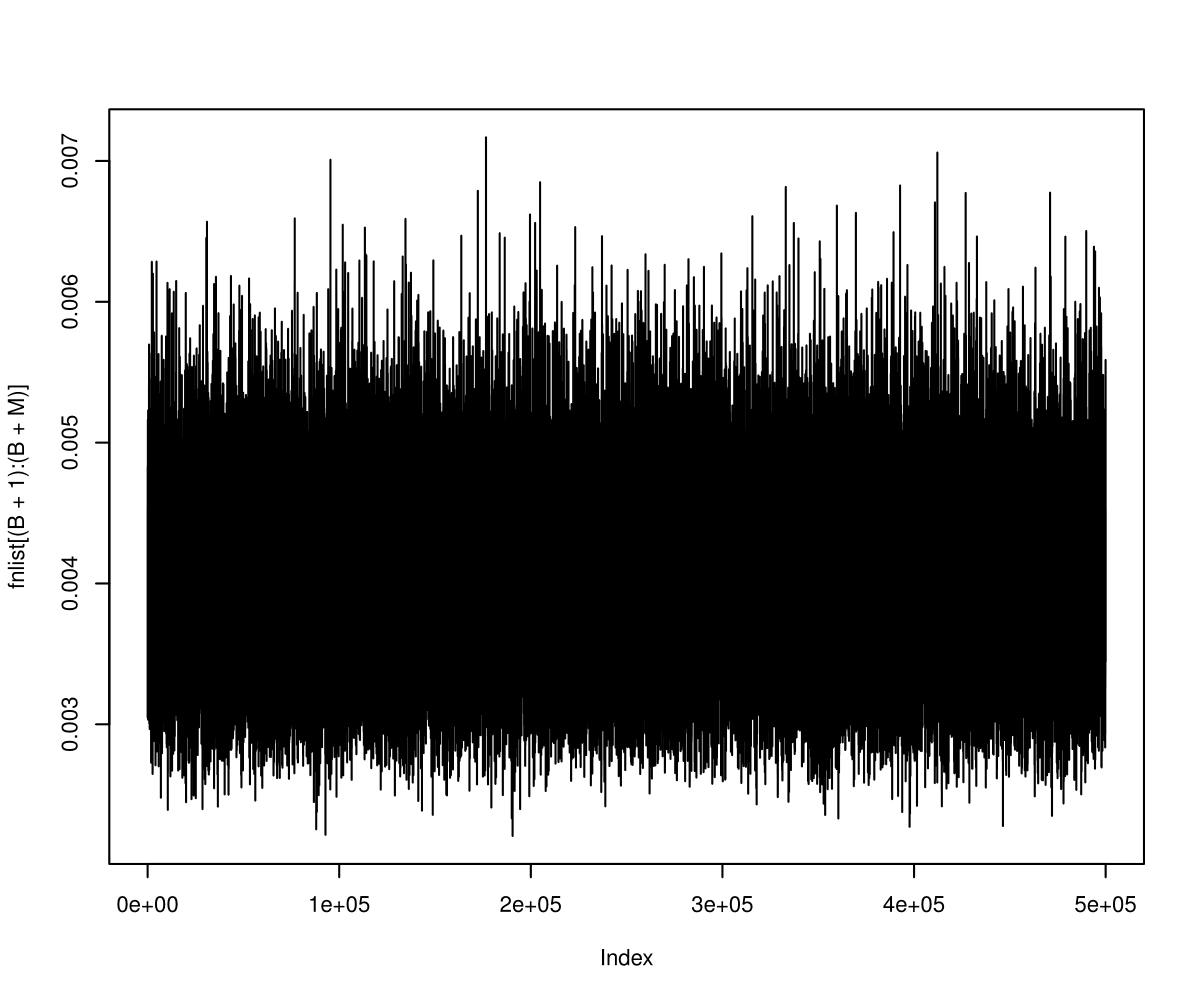
\includegraphics[width=\maxwidth]{figure/p9cplot-1} 

\end{knitrout}
		\caption{function values of Gibbs sampler after burning-in}
\end{figure}
(d) In terms of performance, the Gibbs sampler performs the best among the three as it requires the least amount of burning-in. The random-walk Metropolis requires 2e+6 steps just to burn-in to consistently generates non-trending function values (The function estimates tend to decrease over time if not burnt-in properly). This is quite a waste of computation power. The Metropolis-within-Gibbs requires similar number of steps to burn-in. On the contrary, the Gibbs sampler algorithm requires less than 1e+5 cycles to burn-in, which is magnitudes less than the required burning-in cycles for the other two algorithms. \\
The Gibbs sampler algorithm also performs better in terms of standard error since they produce low varfact values, meaning that the samples generated from the Gibbs sampler algorithm are close to i.i.d. samples. \\
However, the Gibbs sampler requires us to compute the conditional distribution in closed form, which may be very tedious and often impossible. The other two algorithms do not require analytic computation (choosing conjugate priors), hence they are much more easily implemented. \\
The Metropolis-within-Gibbs algorithm converges faster when comparing with the random-walk Metropolis algorithm. This is because the RWM proposes points that differs in all dimensions and will cause a higher chance of rejection.\\
Despite all these disadvantages, there are some advantages to the Random-Walk Metropolis algorithm. For example, if the distribution is defined on two regions that are disconnected in more than one dimension, then the Gibbs-like algorithms will not be able to travel from one region to the other. 
